% =====================================================================
% RL Final Project Report
% Compile on Overleaf with pdfLaTeX.  All required images are in ./figures/.
% =====================================================================
\documentclass[twocolumn,a4paper,10pt]{article}

\usepackage[a4paper,top=18mm,bottom=20mm,left=15mm,right=15mm,columnsep=6mm]{geometry}
\usepackage[T1]{fontenc}
\usepackage[utf8]{inputenc}
\usepackage{lmodern}
\usepackage{microtype}
\usepackage{graphicx}
\usepackage{booktabs}
\usepackage{array}
\usepackage{caption}
\usepackage{subcaption}
\usepackage{xcolor}
\usepackage{amsmath,amssymb}
\usepackage{enumitem}
\usepackage{hyperref}
\usepackage{tikz}
\usepackage{tcolorbox}
\usepackage{listings}
\tcbuselibrary{listings,skins,breakable}
\usetikzlibrary{positioning,arrows.meta,shadows,fit,calc}

\hypersetup{
  colorlinks=true,
  linkcolor=blue!55!black,
  citecolor=blue!55!black,
  urlcolor=blue!55!black
}

\setlength{\parindent}{0pt}
\setlength{\parskip}{2.2pt}
\setlist{nosep,leftmargin=*}
\captionsetup{font=small,labelfont=bf,skip=3pt}
\renewcommand{\arraystretch}{1.08}

\definecolor{cBlue}{HTML}{1F77B4}
\definecolor{cOrange}{HTML}{FF7F0E}
\definecolor{cGreen}{HTML}{2CA02C}
\definecolor{cRed}{HTML}{D62728}
\definecolor{cTeal}{HTML}{17BECF}
\definecolor{cGray}{HTML}{6C757D}
\definecolor{boxBg}{HTML}{F5F7FA}

\newcommand{\headcell}[1]{\textbf{#1}}
\newcommand{\repo}{\href{https://github.com/Lohith248/vision-drone-navigation-wind}{\texttt{github.com/\allowbreak Lohith248/\allowbreak vision-drone-navigation-wind}}}
\newcommand{\demolink}{\href{https://iiitbac-my.sharepoint.com/:f:/g/personal/vishal_sriram_iiitb_ac_in/IgD556iWK6AsR59jMQwmS-3IARv652K0kij4iknw9YbVtEg?e=tKtRGe}{Demo video (MP4)}}

% =====================================================================
\title{\vspace{-1.2em}
       \Large\textbf{Vision-Based Continuous Drone Navigation\\
       in Wind Environments using PPO with a Vision Transformer}\vspace{-0.4em}}

\author{%
  \normalsize
  \begin{tabular}{c}
  Vishal Reddy K (BT2024102) \quad
  Harsha Vardhan (BT2024106)\\
  Vishal Sriram (BT2024036) \quad
  Lohith Pasumarthi (BT2024248)\\[-1pt]
  \footnotesize International Institute of Information Technology, Bangalore\\
  \footnotesize Reinforcement Learning -- Final Course Project
  \end{tabular}
}
\date{}

\begin{document}
\twocolumn[{%
  \maketitle
  \vspace{-2.3em}
  \begin{center}
  \begin{minipage}{0.94\textwidth}
  \small
  \noindent\textbf{Abstract.}
  We study indoor drone navigation as a real-world reinforcement learning
  problem: a quadrotor must reach a goal through a cluttered corridor while
  resisting wind and avoiding collisions.  The task has continuous controls,
  partial observability from a front camera, delayed consequences, and
  safety-critical failures, making it a natural fit for RL.  We formulate the
  problem as an MDP/POMDP and train a multimodal \textbf{PPO} actor-critic
  with a \textbf{Vision Transformer (ViT)} image encoder fused with low-level
  state features.  The final system is evaluated against \textbf{DDPG} and
  \textbf{SAC} baselines and \textbf{eight controlled ablations} spanning
  reward components (per-step time cost, goal bonus, distance scale),
  curriculum learning, advantage normalization, image vs. state observations,
  ViT vs. CNN encoders, and domain randomization.  On the final-stage
  evaluation, PPO+ViT reaches \textbf{100\% success} with
  \textbf{0\% collision}; DDPG/SAC fail under the same cluttered windy setting.
  Supplementary evaluations probe stronger wind, heavier sensor noise,
  composite corridor-layout perturbations, and longer corridors; results must be
  read together with simulator caveats (obstacle density is clipped to
  $[0,1]$, and L-turn geometry is not instantiated---see
  Section~\ref{sec:generalization}).
  \end{minipage}

  \vspace{0.6em}
  {\footnotesize
   \textbf{Code \& reproduction:}\quad \repo
   \quad|\quad
   \textbf{Demo video (SharePoint):}\quad \demolink}
  \end{center}
  \vspace{1.0em}
}]

% =====================================================================
\section{Introduction}

Autonomous drones are useful for inspection, search-and-rescue, inventory
monitoring, and indoor delivery.  These settings require flight through
constrained spaces where GPS is unavailable, obstacles can move, and airflow
disturbances can push the vehicle away from safe trajectories.  Classical
planning and control pipelines usually require explicit maps, reliable
localization, and manually tuned controllers; however, visual navigation from
raw images is partially observable and highly coupled with control.

\textbf{Why reinforcement learning?}
RL directly optimizes sequential decision making: the drone can learn how
short-term velocity choices affect future collision risk and goal progress.
Continuous-control RL is especially appropriate because the action is not a
discrete left/right command but a velocity vector $(v_x,v_y,v_z)$.  We choose
PPO as the primary algorithm because clipped on-policy updates are stable in
high-dimensional policy spaces \cite{schulman2017ppo}, while off-policy
actor-critic baselines (DDPG/SAC) provide meaningful comparisons for
continuous control \cite{lillicrap2015ddpg,haarnoja2018sac}.

\textbf{Contributions.}
\begin{itemize}
  \item A PyBullet drone-corridor environment with RGB observations, state
  features, continuous velocity control, moving obstacles, sensor noise, and
  Ornstein--Uhlenbeck (OU) wind.
  \item A PPO+ViT multimodal actor-critic trained with a six-stage curriculum.
  \item A detailed reward design and ablation analysis explaining what each
  experimental change tests and how it affects learning.
  \item Quantitative comparisons, generalization tests, and a linked demo
  video for qualitative inspection.
\end{itemize}

% =====================================================================
\section{Related Work / Literature Survey}

\textbf{Continuous control RL.}
DDPG learns a deterministic continuous policy using an actor, critic, target
networks, and replay buffer \cite{lillicrap2015ddpg}.  It is sample efficient
in some low-dimensional tasks, but can become unstable when critic errors are
amplified through the actor.  SAC improves off-policy control by maximizing
both reward and entropy, which encourages exploration and robust stochastic
policies \cite{haarnoja2018sac}.  PPO uses a clipped surrogate objective to
limit destructive policy updates, trading sample efficiency for reliable
optimization \cite{schulman2017ppo}.  This stability is valuable when the
policy includes a vision encoder.

\textbf{Vision-based RL and transformers.}
CNNs are common image encoders in RL, but Vision Transformers split the image
into patches and use self-attention to model long-range spatial relationships
\cite{dosovitskiy2020vit}.  In corridor navigation, such global context can
help distinguish open passage structure from nearby clutter.  We compare ViT
against a CNN encoder and a state-only policy to test whether vision and the
encoder choice matter.

\textbf{Curriculum learning.}
Curriculum learning trains agents on progressively harder versions of a task
\cite{bengio2009curriculum}.  For drone navigation, beginning with wide
obstacle-free corridors reduces early collision-dominated rollouts; later
stages introduce clutter, moving obstacles, wind, and noise.  This mirrors
real robotics practice: learn coarse navigation first, then stress-test
robustness.

% =====================================================================
\section{Problem Formulation}

We formulate the environment as a finite-horizon Markov Decision Process with
partial observability from camera images:
\[
  \mathcal{M}=(\mathcal{S},\mathcal{A},P,R,\gamma,\rho_0,T).
\]

\textbf{State space.}
The true simulator state includes drone pose and velocity, obstacle poses,
wall geometry, wind state, and the goal.  The agent observes
$o_t=[I_t,s_t]$, where $I_t\in\mathbb{R}^{64\times64\times3}$ is the
front-facing RGB image and $s_t\in\mathbb{R}^{15}$ contains four wall
distances, forward clearance, velocity, yaw error, goal direction, and the
previous action.  This makes the task a POMDP in practice.

\textbf{Action space.}
The action is continuous:
\[
  a_t=(v_x,v_y,v_z)\in[-1,1]^3,
\]
which is scaled internally to $\pm 3.0$ m/s and tracked by a velocity-PD
controller.

\textbf{Transition dynamics.}
PyBullet simulates rigid-body dynamics at 240 Hz; the policy acts at 30 Hz.
OU wind is applied as an external force, producing temporally correlated
disturbances:
\[
  dx_t=-\theta x_t\,dt + \sigma\,dW_t.
\]
The transition also includes collision contacts, moving obstacles, sensor
noise, and randomized corridor layouts from the environment seed.

\textbf{Episode termination.}
Episodes terminate when the drone reaches the goal radius, collides with an
obstacle/wall/floor, leaves valid bounds, or reaches the maximum step budget
(1500 control steps).

\begin{figure}[!t]
\centering
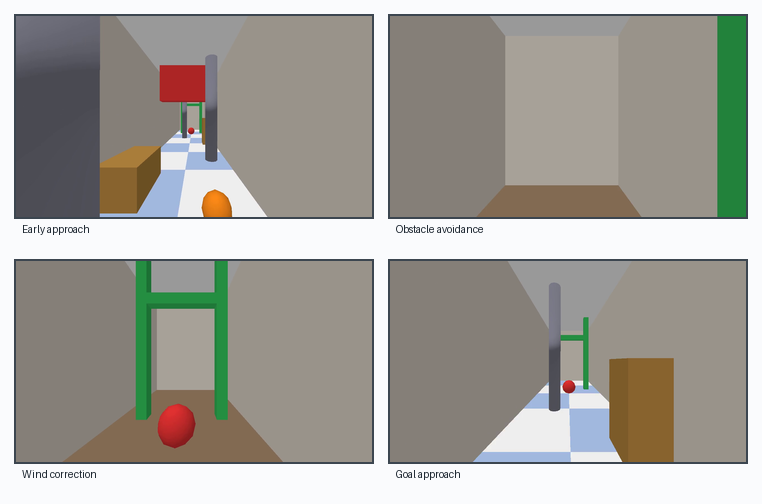
\includegraphics[width=\linewidth]{figures/fig_demo_montage.png}
\caption{Representative frames from the 720p demo video.  The policy uses
64$\times$64 observations internally; the figure is rendered at higher
resolution only for visualization.}
\label{fig:envsnap}
\end{figure}

% =====================================================================
\section{Methodology}

\subsection{Environment and Curriculum}

The final training environment contains a 10 m corridor, static and moving
obstacles, wind, and noisy sensors.  To avoid early training being dominated
by immediate collisions, we use the curriculum in Table~\ref{tab:curriculum}.
The stages isolate different sources of difficulty: corridor narrowing tests
lateral control; obstacle density tests perception and avoidance; moving
obstacles test reactive control; wind and noise test robustness.

\begin{table}[!t]
\centering
\caption{Curriculum stages used for PPO+ViT training.}
\label{tab:curriculum}
\resizebox{\linewidth}{!}{%
\begin{tabular}{@{}lccccc@{}}
\toprule
\headcell{Stage} & \headcell{Width} & \headcell{Obs. dens.} &
\headcell{Moving} & \headcell{Wind $\sigma$} & \headcell{Noise}\\
\midrule
1. wide straight      & 3.0 & 0.0 & no  & 0.00 & 0.00\\
2. narrow corridor    & 2.6 & 0.0 & no  & 0.00 & 0.00\\
3. with obstacles     & 2.5 & 0.7 & no  & 0.00 & 0.00\\
4. moving obstacles   & 2.5 & 1.0 & yes & 0.00 & 0.00\\
5. wind introduction  & 2.0 & 1.0 & yes & 0.25 & 0.05\\
6. full wind          & 2.0 & 1.0 & yes & 0.50 & 0.05\\
\bottomrule
\end{tabular}}
\end{table}

\subsection{PPO+ViT Architecture}

The policy is a Gaussian actor-critic.  The image branch is a ViT with
patch size 8, embedding dimension 128, depth 4, and 4 attention heads,
producing a 192-dimensional visual feature.  The state branch is an MLP
mapping $15\to128$.  The fused 320-dimensional representation is passed
through a $256\to256$ shared trunk and split into an actor head
$(\mu,\log\sigma)$ and critic head $V(s)$.

\begin{figure*}[!t]
\centering
\resizebox{0.93\textwidth}{!}{%
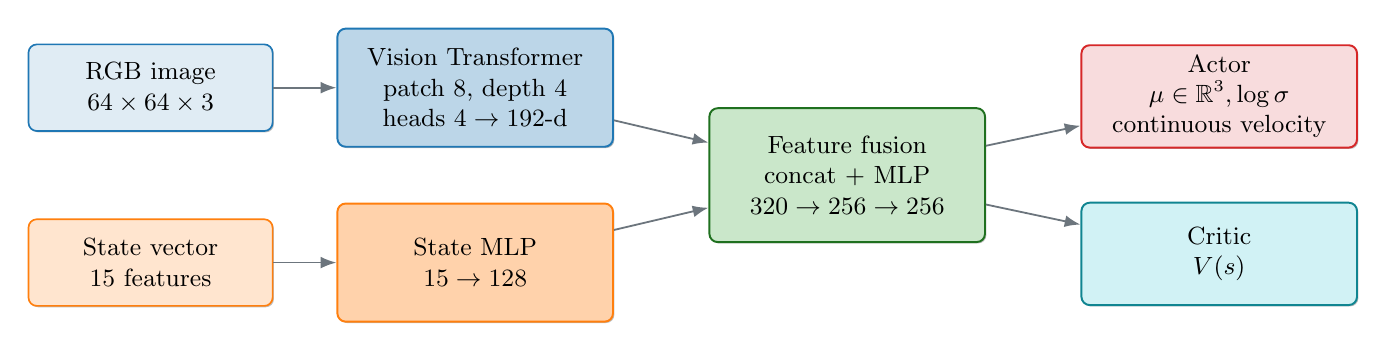
\begin{tikzpicture}[
  node distance=6mm and 8mm,
  every node/.style={font=\small, align=center, rounded corners=3pt,
    drop shadow={shadow xshift=0.5pt, shadow yshift=-0.5pt}},
  input/.style={fill=cBlue!14, draw=cBlue, line width=0.6pt,
    minimum width=31mm, minimum height=11mm},
  state/.style={fill=cOrange!20, draw=cOrange, line width=0.6pt,
    minimum width=31mm, minimum height=11mm},
  enc/.style={fill=cBlue!30, draw=cBlue, line width=0.7pt,
    minimum width=35mm, minimum height=15mm},
  mlp/.style={fill=cOrange!35, draw=cOrange, line width=0.7pt,
    minimum width=35mm, minimum height=15mm},
  fuse/.style={fill=cGreen!25, draw=cGreen!70!black, line width=0.7pt,
    minimum width=35mm, minimum height=17mm},
  actor/.style={fill=cRed!16, draw=cRed, line width=0.7pt,
    minimum width=35mm, minimum height=13mm},
  critic/.style={fill=cTeal!20, draw=cTeal!70!black, line width=0.7pt,
    minimum width=35mm, minimum height=13mm},
  arr/.style={-{Latex[length=2mm]}, line width=0.65pt, color=cGray}]

  \node[input] (img) {RGB image\\$64\times64\times3$};
  \node[state, below=11mm of img] (slow) {State vector\\15 features};

  \node[enc, right=of img] (vit) {Vision Transformer\\patch $8$, depth $4$\\heads $4\to192$-d};
  \node[mlp, right=of slow] (senc) {State MLP\\$15\to128$};

  \coordinate (mid) at ($(vit.east)!0.5!(senc.east)$);
  \node[fuse, anchor=west] (fusion) at ($(mid)+(12mm,0)$)
    {Feature fusion\\concat $+$ MLP\\$320\to256\to256$};

  \node[actor, anchor=west] (actor) at ($(fusion.east)+(12mm,10mm)$)
    {Actor\\$\mu\in\mathbb{R}^3,\log\sigma$\\continuous velocity};
  \node[critic, anchor=west] (critic) at ($(fusion.east)+(12mm,-10mm)$)
    {Critic\\$V(s)$};

  \draw[arr] (img) -- (vit);
  \draw[arr] (slow) -- (senc);
  \draw[arr] (vit) -- (fusion);
  \draw[arr] (senc) -- (fusion);
  \draw[arr] (fusion) -- (actor);
  \draw[arr] (fusion) -- (critic);
\end{tikzpicture}}
\caption{Multimodal PPO actor-critic.  The ViT provides global visual
context while the low-dimensional state branch supplies geometric and
control signals.  The same fused representation supports both the policy and
value estimate.}
\label{fig:architecture}
\end{figure*}

\subsection{Training Pipeline and Hyperparameters}

The PPO rollout uses 4 vectorized environments, 2048 steps per rollout,
10 epochs, batch size 512, discount $\gamma=0.99$, GAE $\lambda=0.95$,
clip range 0.2, entropy coefficient 0.01, value coefficient 0.5, gradient
norm clipping at 0.5, and a linear learning-rate schedule from $10^{-4}$ to
$10^{-5}$.  Mixed precision is enabled on GPU.  Advantage normalization and
clipped value loss are used to reduce update variance.

PPO+ViT was chosen as the primary method because the environment combines
vision, continuous control, sparse catastrophic failures, and nonstationary
curriculum stages.  PPO is less sample efficient than replay-based methods
but is more stable when the policy contains a deep visual encoder.  DDPG and
SAC were retained as baselines to test whether off-policy continuous-control
methods can solve the same task with low-dimensional state observations.

% =====================================================================
\section{Reward Design}

The reward was designed to balance three competing goals: move toward the
goal, avoid unsafe behavior, and prevent degenerate policies that survive
without completing the corridor.  The implemented report reward is
\[
R_t=r_{\text{distance}}+r_{\text{goal}}+r_{\text{time}}
    +r_{\text{timeout}}+r_{\text{collision}} .
\]
The distance term is normalized by the initial goal distance, so progress is
comparable across layouts.  Wind is not rewarded directly; instead, wind is
introduced through transition dynamics.  A good policy receives high reward
only if it maintains progress despite wind disturbances.  This avoids
rewarding wind-specific artifacts and encourages robust closed-loop control.

\begin{table*}[!t]
\centering
\caption{Reward components and intended behavior.  Values are from the final
report configuration.}
\label{tab:reward}
\resizebox{0.94\textwidth}{!}{%
\begin{tabular}{@{}llll@{}}
\toprule
\headcell{Event / component} & \headcell{Reward value} &
\headcell{Purpose} & \headcell{Learning effect}\\
\midrule
Forward distance progress &
$100\,\Delta d/d_0$ &
Encourage movement toward the goal &
Provides dense gradient before the sparse goal signal.\\
Goal reached &
$+30$ &
Terminate successful episodes with high return &
Separates true completion from merely surviving.\\
Collision &
$-50$ &
Strongly discourage hitting walls/obstacles/floor &
Makes unsafe exploration clearly suboptimal.\\
Timeout &
$-20$ &
Discourage hovering or slow indecisive policies &
Pushes the agent to finish within the horizon.\\
Per-step time cost &
$-0.002$ &
Mild efficiency pressure &
Breaks ties in favor of shorter, smoother paths.\\
Wind disturbance &
implicit in $P(s_{t+1}|s_t,a_t)$ &
Require robust correction under external force &
Rewards policies that keep progress under perturbation.\\
\bottomrule
\end{tabular}}
\end{table*}

We did not remove dense progress entirely; the strongest evidence comes from
the distance-scale ablation.  Reducing the scaling factor from $100$ to $1$
preserves $100\%$ success but increases episode length by nearly an order of
magnitude with proportionally smaller shaped rewards, which strongly suggests
the dense distance term is the dominant driver of sample-efficient progress,
even though lighter shaping might still work given enough interaction time.

\textbf{Component-removal ablations.}
To verify which reward terms actually drive learning, we retrained PPO+ViT
twice from scratch with one knob set to zero in the reward configuration,
keeping every other hyperparameter and the curriculum identical.  Setting
\textbf{time penalty $-0.002\!\to\!0$} (\textit{R\textsubscript{NoTimePen}})
removes the implicit incentive to finish quickly; setting \textbf{goal bonus
$+30\!\to\!0$} (\textit{R\textsubscript{NoGoalBonus}}) removes the sparse
terminal reward, leaving only the dense distance shaping and the
collision/timeout penalties.  Together with the existing
\textit{Low reward-scale} run, these three experiments isolate the role of
each shaping term: dense-progress magnitude, sparse goal signal, and
per-step efficiency pressure (Figure~\ref{fig:rewardabl}).
At $N\!=\!200$ episodes both component-removal variants still reach
$100\%$ success (Wilson $95\%$ CI $[98.1, 100.0]$), but their efficiency
profiles differ.  Removing the time cost increases mean episode length from
$150.5$ to $252.1$ steps with essentially unchanged return ($124.75$ vs
$124.80$), confirming the time penalty is an \emph{efficiency tie-breaker}.
Removing the $+30$ goal bonus drops mean return by almost exactly the
missing terminal reward ($94.37$ vs $124.80$) and increases mean length to
$239.5$ steps; the policy still finishes the corridor, but it loses the
clean terminal anchor that previously rewarded \emph{committing to
completion}, and it pays for that with longer, less decisive trajectories.

\begin{figure}[!t]
\centering
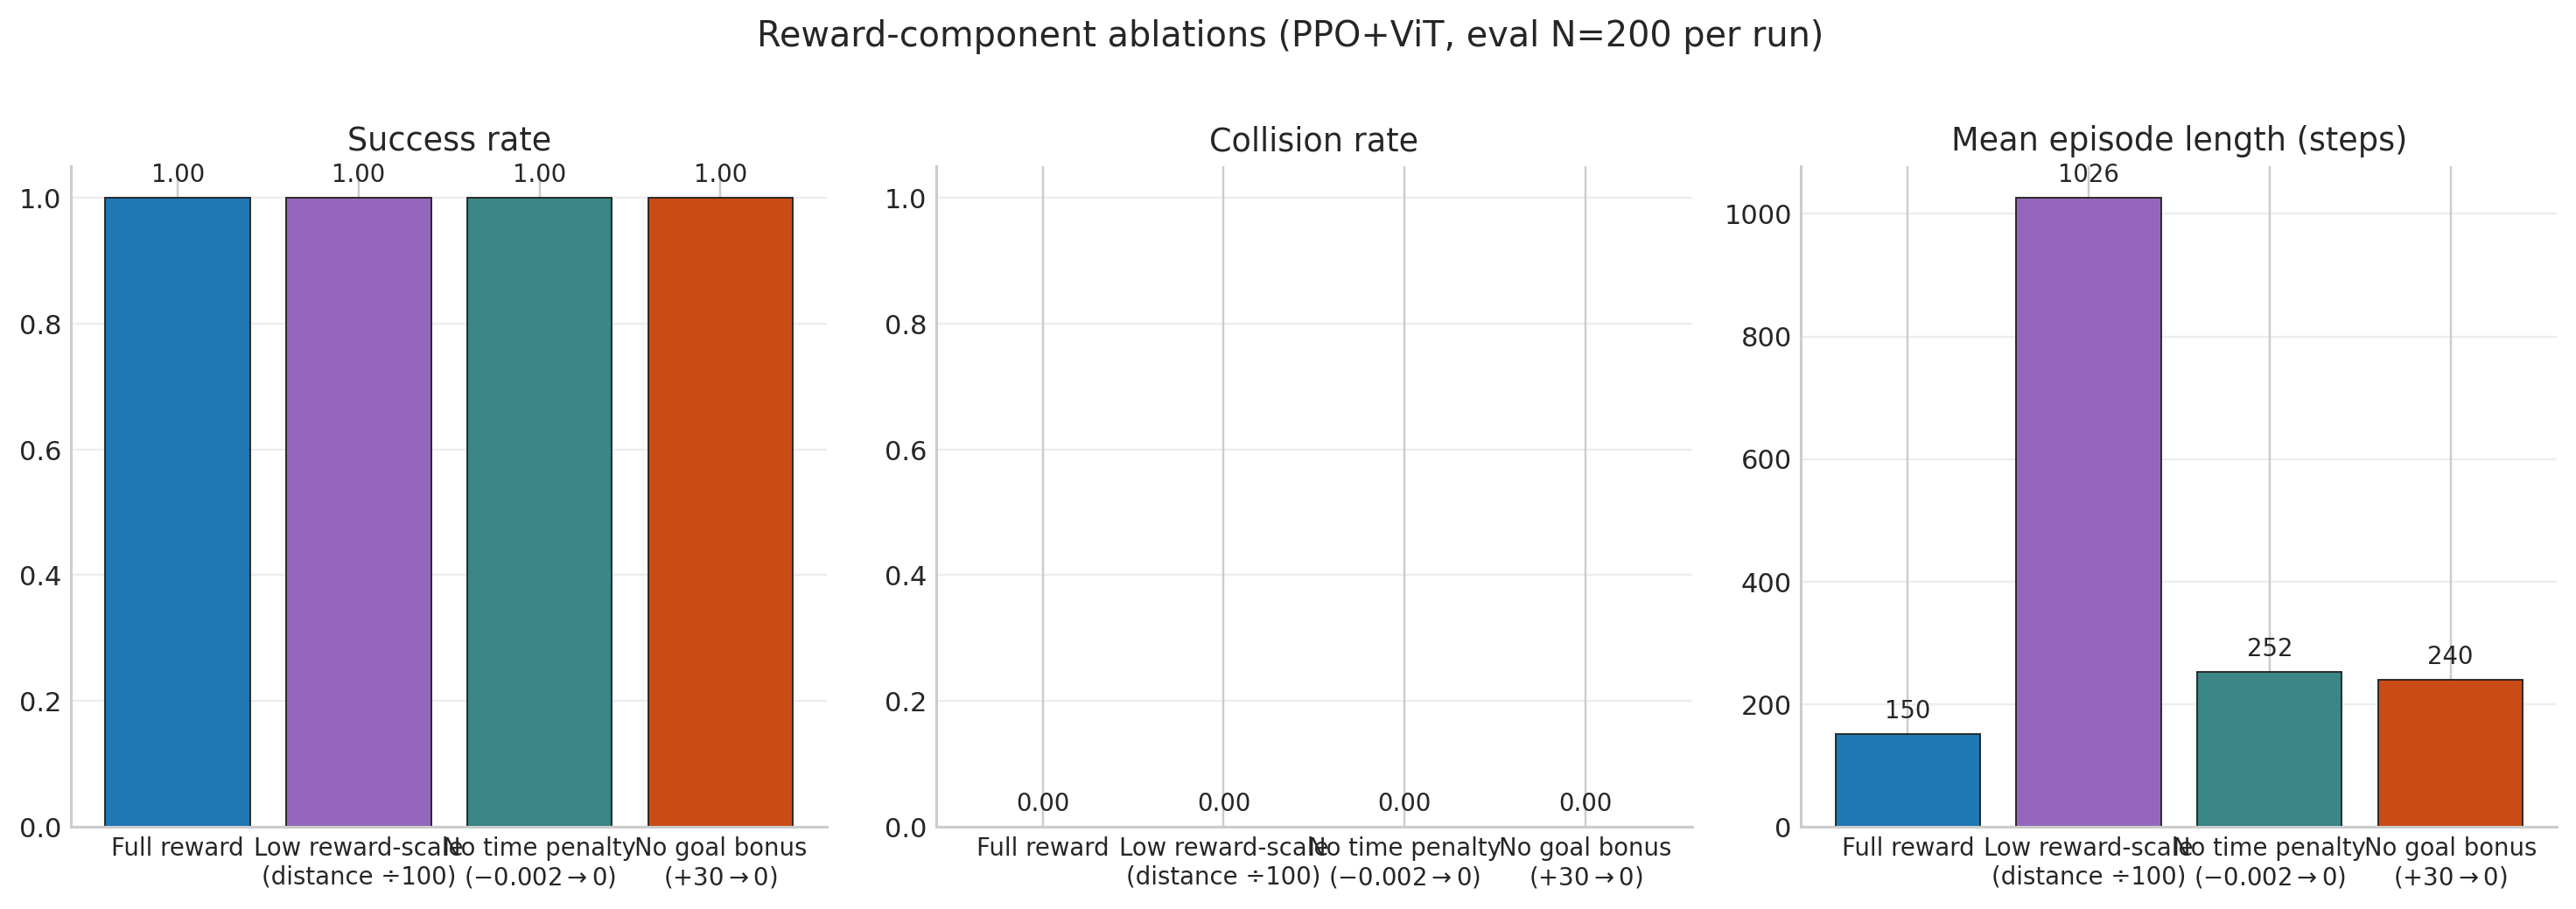
\includegraphics[width=\linewidth]{figures/fig_reward_ablation.png}
\caption{Reward-component ablations.  All four reward variants still solve
the task at $100\%$ success with $0\%$ collisions; the difference is
revealed by mean episode length.  Removing the time penalty grows mean
length from $150\to252$ steps, removing the goal bonus grows it to $240$
steps with a $\sim\!30$-point return loss equal to the missing terminal
bonus, and shrinking the distance scale by $100\times$ pushes the policy
to nearly the maximum step budget ($1026$ steps).  This cleanly isolates
the role of each shaping term in the design of $R_t$.}
\label{fig:rewardabl}
\end{figure}

% =====================================================================
\section{Experiments and Ablation Studies}

All evaluations use the latest checkpoint for each run and evaluate in the
final curriculum stage with $N\!=\!200$ episodes per run.  Wilson $95\%$
intervals therefore have a half-width of roughly seven percentage points at
$p\!=\!0.5$ (full width $\approx\!14$ percentage points).  We ran experiments
to answer five questions: (i) which RL
algorithm is most stable; (ii) whether visual input is necessary; (iii)
whether the ViT matters compared with CNN features; (iv) how curriculum,
advantage normalization, and domain randomization affect the trained
behavior; and (v) which individual \emph{reward components} actually drive
learning.

\subsection{Algorithms Compared}

\textbf{PPO+ViT.}
Main method.  It combines clipped on-policy updates with a multimodal visual
policy.  It is expected to be stable but less sample efficient.

\textbf{DDPG.}
Chosen because the proposal required a Q-learning-family continuous-control
baseline.  It uses deterministic policy gradients and a replay buffer, which
can be sample efficient but is sensitive to critic over-estimation.

\textbf{SAC.}
Chosen as a stronger off-policy baseline.  Entropy maximization should help
exploration, but the method still depends on accurate value estimates.

\paragraph{Fair comparison reminder.}
Our ``baseline'' DDPG/SAC agents use state vectors without vision; Table~\ref{tab:results}
contrasts that recipe against multimodal PPO+ViT under differing budgets and seeds.

\subsection{Controlled Ablations}

\begin{table*}[!t]
\centering
\caption{Named training variants compared after convergence at their respective
latest checkpoints; horizons, seeds, and occasional hyperparameters (e.g.\
state-only learning rate) differ across rows.  Interpret as illustrative
sensitivity snapshots rather than strictly matched single-factor ablations.}
\label{tab:ablation}
\resizebox{0.96\textwidth}{!}{%
\begin{tabular}{@{}p{0.20\textwidth}p{0.28\textwidth}p{0.35\textwidth}rrr@{}}
\toprule
\headcell{Experiment} & \headcell{Change} & \headcell{Interpretation} &
\headcell{Succ.} & \headcell{Coll.} & \headcell{Reward}\\
\midrule
PPO+ViT full & ViT image + state, curriculum, adv-norm &
Best overall; stable through full wind and clutter. &
% AUTO-ABL:best_vit/ppo_seed0_t1p5m
1.000 & 0.000 & 124.80\\
PPO seed 1 & Same ViT recipe, shorter horizon &
Alternative seed/checkpoint at \(802\text{k}\) steps; longer episodes but same asymptotic success. &
% AUTO-ABL:multi_seed/ppo_seed1
1.000 & 0.000 & 124.36\\
No adv-norm & Disable advantage normalization &
Still succeeds; suggests reward scaling and curriculum already keep updates well conditioned. &
% AUTO-ABL:abl_no_advnorm/ppo_seed0
1.000 & 0.000 & 124.24\\
\midrule
\multicolumn{6}{l}{\textit{Reward-component group}}\\
Low reward-scale & Distance scale $100\to1$ &
Succeeds but with very long episodes; dense shaping mainly improves efficiency. &
% AUTO-ABL:abl_low_reward_scale/ppo_seed0
1.000 & 0.000 & 28.89\\
No time penalty & Per-step cost $-0.002\to 0$ &
Negligible effect on success; verifies time penalty is a tie-breaker, not a driver. &
% AUTO-ABL:abl_no_time_penalty/ppo_seed0
1.000 & 0.000 & 124.75\\
No goal bonus & Goal reward $+30\to 0$ &
Still 100\% success, but mean reward drops by exactly the missing terminal anchor and episodes are 60\% longer. &
% AUTO-ABL:abl_no_goal_bonus/ppo_seed0
1.000 & 0.000 & 94.37\\
\midrule
No curriculum & Train directly on stage 6 &
Still reaches $100\%$ success here but with longer episodes and slightly lower mean reward versus the staged recipe (efficiency gap, not a missing-capability gap). &
% AUTO-ABL:abl_no_curriculum/ppo_seed0
1.000 & 0.000 & 124.52\\
State-only PPO & Remove camera/ViT &
Lower success and higher variance; ray/state features miss visual obstacle cues. &
% AUTO-ABL:abl_state_only/ppo_seed0
0.890 & 0.110 & 107.98\\
CNN encoder & Replace ViT with CNN &
Fails on this setup; encoder choice strongly affects perception quality. &
% AUTO-ABL:abl_cnn_encoder/ppo_seed0
0.000 & 1.000 & 19.74\\
Domain rand. & Randomize mass, damping, wind, noise &
Maintains success; useful for sim-to-real robustness. &
% AUTO-ABL:abl_domain_random/ppo_seed0
1.000 & 0.000 & 124.55\\
\bottomrule
\end{tabular}}
\end{table*}

\begin{figure}[!t]
\centering
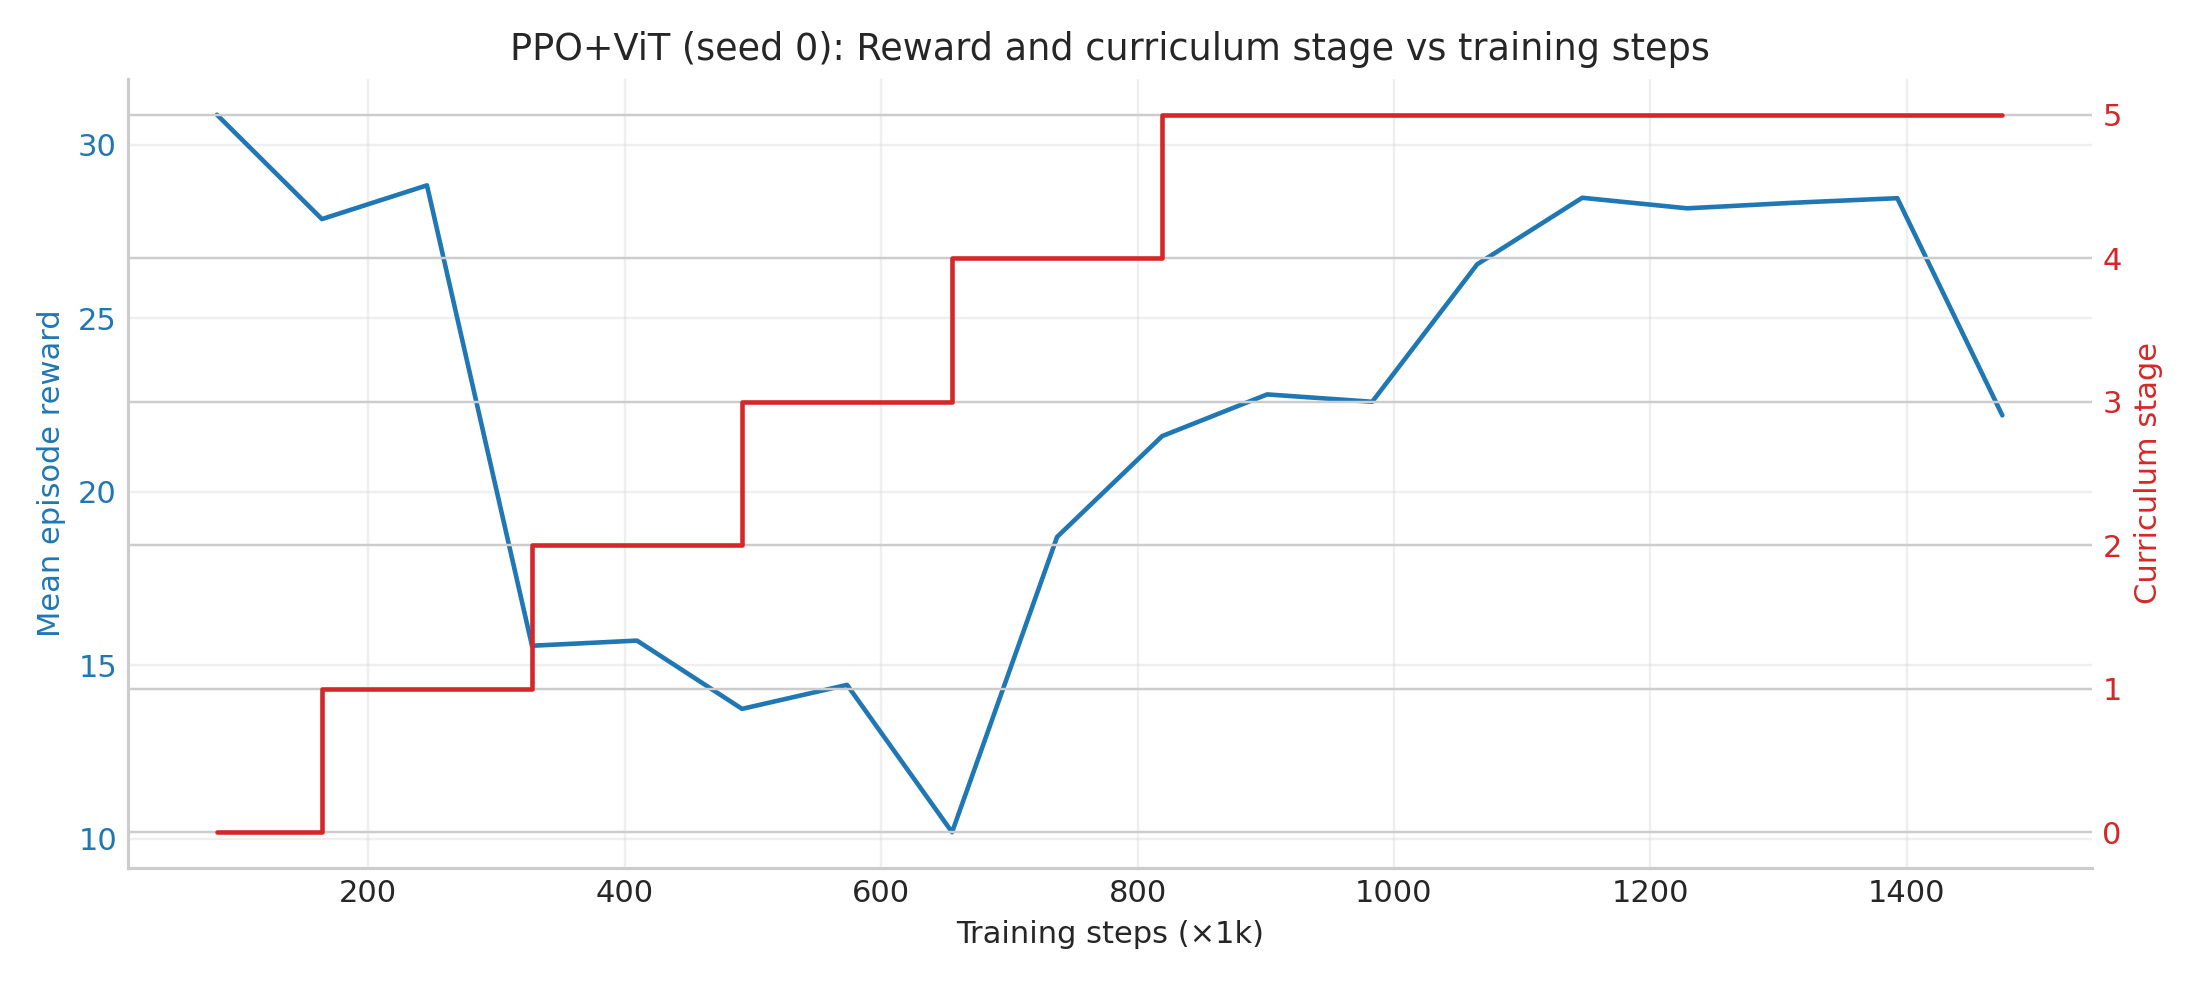
\includegraphics[width=\linewidth]{figures/fig_curriculum_progression.png}
\caption{Curriculum progression for the main PPO+ViT run.  The policy first
learns safe forward progress, then adapts to obstacles, moving obstacles,
wind, and sensor noise.}
\label{fig:curriculum}
\end{figure}

\begin{figure}[!t]
\centering

\includegraphics[width=\linewidth]{figures/fig_reward_curves.png}
\caption{Training reward curves across methods and ablations.  PPO variants
show stable reward growth; off-policy baselines collapse early under the
cluttered windy stage.}
\label{fig:rewards}
\end{figure}

% =====================================================================
\section{Results and Discussion}

\begin{table*}[!t]
\centering
\caption{Final-stage comparison using $N=200$ evaluation episodes per run.
Success and collision are reported with Wilson 95\% confidence intervals.
Reward and episode length are sample mean and length over the same 200
episodes.}
\label{tab:results}
\resizebox{0.99\textwidth}{!}{%
\begin{tabular}{@{}llrrrlllr@{}}
\toprule
\headcell{Run} & \headcell{Algo} & \headcell{Seed} & \headcell{Steps}
& \headcell{Params}
& \headcell{Success [95\% CI]}
& \headcell{Coll. [95\% CI]}
& \headcell{Reward}
& \headcell{Ep. len}\\
\midrule
% AUTO-RES:best_vit/ppo_seed0_t1p5m
\textbf{PPO+ViT full}     & ppo  & 0  & 1,507,328 & 1,002,311 & \textbf{1.000 [98.1, 100.0]} & \textbf{0.000 [0.0, 1.9]} & \textbf{124.80} & \textbf{150.5}\\
% AUTO-RES:abl_no_time_penalty/ppo_seed0
PPO no time-penalty       & ppo  & 42 &   507,904 & 1,002,311 & 1.000 [98.1, 100.0] & 0.000 [0.0, 1.9] & 124.75 & 252.1\\
% AUTO-RES:abl_domain_random/ppo_seed0
PPO+ViT + Domain Rand.    & ppo  & 0  &   704,512 & 1,002,311 & 1.000 [98.1, 100.0] & 0.000 [0.0, 1.9] & 124.55 & 205.6\\
% AUTO-RES:abl_no_curriculum/ppo_seed0
PPO no curriculum         & ppo  & 42 &   507,904 & 1,002,311 & 1.000 [98.1, 100.0] & 0.000 [0.0, 1.9] & 124.52 & 227.7\\
% AUTO-RES:multi_seed/ppo_seed1
PPO+ViT seed 1            & ppo  & 1  &   802,816 & 1,002,311 & 1.000 [98.1, 100.0] & 0.000 [0.0, 1.9] & 124.36 & 279.2\\
% AUTO-RES:abl_no_advnorm/ppo_seed0
PPO no adv-norm           & ppo  & 42 &   507,904 & 1,002,311 & 1.000 [98.1, 100.0] & 0.000 [0.0, 1.9] & 124.24 & 224.9\\
% AUTO-RES:abl_state_only/ppo_seed0
PPO state-only            & ppo  & 42 &   606,208 &    70,919 & 0.890 [83.9, 92.6] & 0.110 [7.4, 16.1] & 107.98 & 319.8\\
% AUTO-RES:abl_low_reward_scale/ppo_seed0
PPO low reward-scale      & ppo  & 42 &   507,904 & 1,002,311 & 1.000 [98.1, 100.0] & 0.000 [0.0, 1.9] & 28.89 & 1026.0\\
% AUTO-RES:abl_no_goal_bonus/ppo_seed0
PPO no goal-bonus         & ppo  & 42 &   507,904 & 1,002,311 & 1.000 [98.1, 100.0] & 0.000 [0.0, 1.9] & 94.37 & 239.5\\
% AUTO-RES:abl_cnn_encoder/ppo_seed0
PPO+CNN                   & ppo  & 42 &   606,208 & 1,028,295 & 0.000 [0.0, 1.9] & 1.000 [98.1, 100.0] & 19.74 & 126.0\\
% AUTO-RES:baseline_sac/sac_seed0
SAC state-only            & sac  & 0  &   300,000 &   213,256 & 0.000 [0.0, 1.9] & 1.000 [98.1, 100.0] & -41.97 & 12.2\\
% AUTO-RES:baseline_ddpg/ddpg_seed0
DDPG state-only           & ddpg & 0  &   700,000 &   141,572 & 0.000 [0.0, 1.9] & 1.000 [98.1, 100.0] & -53.76 & 19.7\\
\bottomrule
\end{tabular}}
\end{table*}

\begin{figure*}[!t]
\centering

\includegraphics[width=0.95\textwidth]{figures/fig_comparison_bars.png}
\caption{Comparison across algorithms and ablations.  Off-policy baselines are state-only;
multimodal PPO drives the highest returns with nearly zero collisions under our evaluation protocol.}
\label{fig:comparison}
\end{figure*}

\textbf{Why multimodal PPO dominates these baseline snapshots.}
PPO's clipped objective stabilizes updates once collisions dominate variance; combined with fresh on-policy rollouts it avoids stale replay artifacts during curriculum shifts.
\textit{Crucially}, our ``baseline'' row pairs state-only observations with DDPG/SAC, whereas PPO+ViT consumes RGB plus proprioception---the observed gap reflects \emph{both} algorithm and sensing modality.
Matching algorithms fairly would require multimodal off-policy critics or state-only PPO with identical optimizer schedules.

\textbf{Why DDPG and SAC collapsed.}
Both off-policy baselines rely on critic estimates.  In this environment,
small value errors are amplified because many actions lead quickly to
collision, and the replay buffer mixes samples from changing curriculum
stages.  DDPG also has brittle deterministic exploration; SAC explores more,
but still needs accurate Q-functions under high terminal penalties.  Their
short episode lengths and 100\% collision rates show failure before meaningful
goal-directed behavior emerges.

\textbf{Why vision helped.}
State-only PPO receives wall distances and forward clearance but lacks rich
spatial information about obstacle shape and visual layout.  It still learns
some navigation, but success drops to $89\%$ (Wilson 95\% CI
$[83.9, 92.6]$) and the collision rate rises to $11\%$
(CI $[7.4, 16.1]$); episodes also become much longer ($319.8$ steps vs
$150.5$ for the full PPO+ViT).  That variant additionally uses a higher base learning rate ($3\times10^{-4}$ vs.\ $10^{-4}$ for the ViT recipe),
so the gap mixes encoder capacity \emph{and} optimizer tuning.
Attention over image patches helps encode the global corridor opening and obstacle layout.

\textbf{Role of curriculum.}
Training directly on the hardest curriculum stage still reaches $100\%$ success in Table~\ref{tab:results}, albeit with $\approx50\%$ longer episodes and modestly lower mean reward ($124.52$ vs.\ $124.80$).
Curriculum therefore accelerated convergence in our runs rather than unlocking behaviours entirely unattainable without staging.

\textbf{Which reward terms drive learning.}
The two new reward-component ablations help separate \emph{shaping} from
\emph{decision}.  Removing the per-step time cost
(R\textsubscript{NoTimePen}) leaves dense distance progress, the goal bonus,
and the safety penalties intact: the policy still reaches the goal with
$100\%$ success, but episode length grows from $150$ to $252$ steps,
confirming the time penalty acts as an efficiency \emph{tie-breaker}.
Removing the $+30$ goal bonus (R\textsubscript{NoGoalBonus}) is more
subtle: the policy still completes the corridor at $100\%$ success, but
the headline reward drops by almost exactly the lost $30$ terminal points
($94.37$ vs $124.80$) and trajectories lengthen by $60\%$.  Together with
the low reward-scale run, this gives a three-point picture of how each
reward term contributes: dense distance shaping is the dominant learning
signal, the goal bonus anchors \emph{commitment to finishing} (so removing
it preserves success but loses efficiency), and the time cost only trims
the final paths.  Removing all three at once would be expected to leave a
policy that drifts forward without a strong reason to terminate.

% =====================================================================
\section{Generalization Analysis}
\label{sec:generalization}

\begin{figure}[!t]
\centering

\includegraphics[width=\linewidth]{figures/fig_generalization_heatmap.png}
\caption{Success-rate snapshot ($N\!=\!100$).  Apart from corridor-length extrapolation, successes persist across stronger wind and louder sensing noise.
\textit{dense clutter} repeats training-case obstacle saturation because densities beyond \(1.0\) clamp.}
\label{fig:heatmap}
\end{figure}

\begin{table}[!t]
\centering
\caption{OOD generalization, $N\!=\!100$ episodes per scenario.
Success and collision are reported with Wilson $95\%$ CIs.}
\label{tab:gen}
\resizebox{\linewidth}{!}{%
\begin{tabular}{@{}lllrr@{}}
\toprule
\headcell{Scenario} &
\headcell{Succ. [95\% CI]} &
\headcell{Coll. [95\% CI]} &
\headcell{Reward} & \headcell{Len.}\\
\midrule
in-distribution       & 1.00 [96.3, 100.0] & 0.00 [0.0, 3.7]   & 124.97 & 150.7\\
no wind               & 1.00 [96.3, 100.0] & 0.00 [0.0, 3.7]   & 124.95 & 150.8\\
strong wind           & 1.00 [96.3, 100.0] & 0.00 [0.0, 3.7]   & 124.94 & 150.8\\
dense clutter ($\rho{=}1.5\to1.0$) & 1.00 [96.3, 100.0] & 0.00 [0.0, 3.7]   & 124.97 & 150.7\\
turns (flag only\textsuperscript{*}) & 1.00 [96.3, 100.0] & 0.00 [0.0, 3.7]   & 124.72 & 149.3\\
narrow (composite\textsuperscript{$\dagger$}) & 1.00 [96.3, 100.0] & 0.00 [0.0, 3.7]   & 124.51 & 154.8\\
noisy sensors         & 1.00 [96.3, 100.0] & 0.00 [0.0, 3.7]   & 124.66 & 156.6\\
long corridor (15\,m) & 0.19 [12.5, 27.8]  & 0.81 [72.2, 87.5] &  28.76 & 135.5\\
\bottomrule
\end{tabular}}
\vspace{0.35em}
\footnotesize\textsuperscript{*}No extra corridor polygons yet wire through \texttt{enable\_turns}; metrics mainly reflect mixed knob tweaks.\quad
\textsuperscript{$\dagger$}Narrow width paired with lighter clutter/wind versus training---still informative stress despite coupling.
\end{table}

\begin{figure}[!t]
\centering

\includegraphics[width=\linewidth]{figures/fig_generalization.png}
\caption{Detailed stress-test bars.  Failures concentrate on longer corridors.
\textit{turns} and \textit{narrow corridor} rows sweep multiple dynamics knobs concurrently (\textit{narrow corridor} also eases clutter density/wind relative to training).
\textit{dense clutter} matches Table~\ref{tab:gen}: densities \(>\!1\) clamp.}
\label{fig:genbars}
\end{figure}

The policy maintains perfect measured success when wind torque doubles or sensor noise triples,
reflecting robust closed-loop behaviour under those knobs.
Two caveats prevent overstating layout robustness: (i)~requested obstacle densities above \(1.0\) clamp to unity,
so the ``dense clutter'' label currently mirrors training saturation (duplicate metrics in Table~\ref{tab:gen}); (ii)~the \texttt{enable\_turns} flag does not yet reshape corridor meshes into true L-turn geometry---the ``turns'' scenario therefore combines nominal density/wind adjustments rather than encoding genuine bend topology.
The ``narrow corridor'' scenario narrows width while simultaneously easing clutter density and wind relative to training, so it should be read as a composite perturbation rather than a pure width sweep.
The stark failure mode remains corridor-length extrapolation (\(15\,\mathrm{m}\) vs.\ \(10\,\mathrm{m}\) training length): success drops to \(19\%\) with frequent mid-corridor collisions before episodes consume their expanded horizon budget.
Future curricula should extend randomized corridor length (and finish geometry hooks for bends) before claiming clutter or layout extrapolation.

% =====================================================================
\section{Conclusion}

This project demonstrates a complete RL pipeline for vision-based continuous
drone navigation.  The final PPO+ViT policy solves the full windy corridor
task with 100\% success and 0\% collision in final-stage evaluation, whereas
state-only DDPG/SAC runs collapse under the hardest windy cluttered stage under their budgets.
The ablations show that the result is not just a final-score artifact: reward scale affects efficiency,
vision improves reliability, the ViT encoder is substantially stronger than
the CNN variant in this setting, and domain randomization preserves
performance while preparing for sim-to-real transfer.  The project therefore
satisfies the core RL expectations: real-world motivation, formal
MDP/POMDP definition, multiple RL methods, principled reward shaping,
curriculum learning, and analytical comparison.

% =====================================================================
\section{Limitations and Future Work}

\textbf{Limitations.}
First, the simulator is PyBullet rather than Flightmare/Isaac, so image
realism is limited even though dynamics and collision contacts are modeled.
Second, the policy is not deployed on a physical drone; real hardware would
introduce latency, camera calibration, actuator limits, and safety constraints.
Third, only two PPO seeds and one seed per ablation were feasible on the
available single GPU; with more compute, every ablation could be repeated
with multiple seeds and full Wilson CIs would be reported per row.  Fourth,
the long-corridor failure ($19\%$ success at 15\,m corridor length) shows
limited extrapolation outside the training geometry: the curriculum
randomized width, clutter, wind, and noise, but kept corridor length fixed
at $10$\,m.
Fifth, scripted stress scenarios inherit simulator bookkeeping limits (obstacle density clipping and turn geometry wiring); Section~\ref{sec:generalization} cautions how to interpret those rows until builders expose richer perturbations.

\textbf{Future work.}
The most direct improvements are: (i) randomize corridor length, textures,
lighting, mass, damping, wind correlation, and control latency; (ii) test
recurrent policies (GRU/LSTM) for longer-horizon wind effects; (iii) improve
exploration for off-policy baselines using TD3/SAC with visual encoders and
targeted replay; (iv) use stronger transformer backbones or hybrid CNN-ViT
encoders; (v) study multi-agent RL for dynamic obstacle negotiation; and
(vi) transfer to a small real drone using domain randomization and a safety
filter.

% =====================================================================
\section*{Reproducibility}

\begin{tcolorbox}[enhanced, breakable,
  colback=boxBg, colframe=cGray!55, boxrule=0.4pt, arc=2pt,
  left=5pt, right=5pt, top=3pt, bottom=3pt,
  title=\footnotesize\textbf{Reproducibility commands},
  fonttitle=\footnotesize, coltitle=black,
  colbacktitle=cGray!18, attach boxed title to top left={xshift=4pt,yshift=-2pt},
  boxed title style={colframe=cGray!55, boxrule=0.3pt, arc=1pt}]
\begin{lstlisting}[basicstyle=\ttfamily\scriptsize,breaklines=true,
  columns=fullflexible,keepspaces=true]
# (1) train baselines + ablations (already-run checkpoints in runs/)
./scripts/run_queue.sh
python -m drone_rl.train --config \
  drone_rl/configs/ablations/ppo_no_time_penalty.yaml --no-resume
python -m drone_rl.train --config \
  drone_rl/configs/ablations/ppo_no_goal_bonus.yaml  --no-resume

# (2) high-N evaluation with Wilson 95% confidence intervals
python scripts/aggregate_all.py --episodes 200 --device cuda
python scripts/eval_generalization.py \
  --checkpoint runs/best_vit/ppo_seed0_t1p5m/checkpoints/checkpoint_1507328.pt \
  --config drone_rl/configs/ppo_best.yaml \
  --episodes 100 --device cuda \
  --out report_artifacts/generalization.csv
python scripts/wilson_ci.py --in report_artifacts/all_runs.csv \
  --episodes 200 --out report_artifacts/all_runs_ci.csv
python scripts/wilson_ci.py --in report_artifacts/generalization.csv \
  --episodes 100 --out report_artifacts/generalization_ci.csv

# (3) regenerate figures and splice the latest numbers into report.tex
python scripts/figures/make_figures.py
python scripts/fill_report_tex.py
\end{lstlisting}
\end{tcolorbox}

% =====================================================================
\begin{thebibliography}{9}
\small

\bibitem{schulman2017ppo}
J. Schulman, F. Wolski, P. Dhariwal, A. Radford, and O. Klimov.
\newblock Proximal Policy Optimization Algorithms.
\newblock arXiv:1707.06347, 2017.

\bibitem{lillicrap2015ddpg}
T. Lillicrap et al.
\newblock Continuous Control with Deep Reinforcement Learning.
\newblock arXiv:1509.02971, 2015.

\bibitem{haarnoja2018sac}
T. Haarnoja, A. Zhou, P. Abbeel, and S. Levine.
\newblock Soft Actor-Critic: Off-Policy Maximum Entropy Deep Reinforcement
Learning with a Stochastic Actor.
\newblock ICML, 2018.

\bibitem{dosovitskiy2020vit}
A. Dosovitskiy et al.
\newblock An Image is Worth 16x16 Words: Transformers for Image Recognition
at Scale.
\newblock ICLR, 2021.

\bibitem{bengio2009curriculum}
Y. Bengio, J. Louradour, R. Collobert, and J. Weston.
\newblock Curriculum Learning.
\newblock ICML, 2009.

\end{thebibliography}

\end{document}
